\documentclass{report}

\usepackage{amsmath}
\usepackage{amssymb}
\usepackage{array}
\usepackage{mathtools}
\usepackage{titlepic}
\usepackage{url}
\usepackage{natbib}
\usepackage{graphicx}
\usepackage{listings}
\usepackage{color}
\usepackage{lmodern}
%\usepackage{nicefrac}
\usepackage{xfrac}
\usepackage[T1]{fontenc}

\setlength\parindent{0pt}
\graphicspath{{./images/}}

\renewcommand{\baselinestretch}{1.5}







\begin{document}

\titlepic{
\includegraphics[scale=0.5]{DIT_logocol}}
\title{Discrete Population Models for Single Species}
\author{Jerry Kiely\\
	\\
	School of Mathematical Sciences\\
	Dublin Institute of Technology\\
	Dublin 8\\
	Ireland\\
	\\
	\texttt{d16126734@mydit.ie}}
\date{\today}
\maketitle


\tableofcontents

%\thispagestyle{empty}
\newpage

\begin{minipage}[b]{1\linewidth}
    \listoffigures
\end{minipage}

\begin{minipage}[b]{1\linewidth}
    \listoftables
\end{minipage}

%\lstlistoflistings

\newpage










\begin{abstract}
The author presents a review of \emph{Discrete Population Models for Single Species}. He
describes their relevance and applications, gives a graphical approach to solving non-linear
models, presents some of the details around \emph{Equilibrium}, \emph{Stability}, and
\emph{Chaos}, looks rigorously at the technique of \emph{Linearisation} around equilibrium
points, and then reviews \emph{Discrete Models with Delay}.
\end{abstract}









%\chapter{Significance and applications}
\chapter{Discrete Models}




\section{Introduction}

Discrete models, as opposed to continuous models, use difference equations (rather than differential equations) to
model biological phenomena, such as populations, when it makes sense to measure the interval of time between events
as discrete or fixed. It also makes sense where successive measurements occur at fixed time intervals - such as
census data. We are interested in models of the form: \bigskip

\[
	x_{t + 1} = f(x_t)
\]\medskip

Where $f$ is a linear or non-linear function of $x_t$. The sequence $\{x_0, x_1, x_2, \ \ldots \ \}$ is called
the \emph{orbit}. \bigskip

As an example, consider a population that changes over time through births and deaths only. Let us denote the population
at time $t$ to be $x_t$, and the population at time $t + 1$ to be $x_{t + 1}$. With a birth rate $r_b$ and a death rate
$r_d$, we can describe the rate of change of the population as follows: \bigskip

\begin{eqnarray*}
  x_{t + 1} - x_t & = & r_b x_t - r_d x_t \\
                  & = & (r_b - r_d) x_t \\
        x_{t + 1} & = & x_t + (r_b - r_d) x_t \\
                  & = & (1 + r_b - r_d) x_t \\
                  & = & r x_t
\end{eqnarray*}\medskip

where $r = 1 + r_b - r_d$. From here it is easy to show that: \bigskip

\begin{eqnarray*}
    x_t & = & r x_{t - 1} \\
        & = & r (r x_{t - 2}) \\
        & = & r^2 x_{t - 2} \\
        & = & r^2 (r x_{t - 3}) \\
        & = & r^3 x_{t - 3} \\
        & \mathrel{\makebox[\widthof{=}]{\vdots}} \\
        & = & r^t x_0
\end{eqnarray*}\medskip

and for this simple model it is clear to see that when $\left| r \right| < 1$ then the population decays to zero,
and if $\left| r \right| > 1$ then the population grows without bound. If $\left| r \right| = 1$ then the
population exhibits no growth or decay at all, remaining constant at it's initial value. \bigskip




\section{Applications}

Some examples where discrete models may be used are: \bigskip

\begin{itemize}
	\item plant population (annual reproduction)
	\item insect population (where there is no overlap in generations)
	\item cell population (within a culture)
\end{itemize}\medskip




\section{Solutions}

Solving a linear discrete model - coming up with a formula that expresses the $n$-th
iterate of our model in terms of the parameters of the model - is easy, and allows us
to make long-term predictions about the behaviour of our model. In the non-linear case
it is not possible to do this, and hence difficult to make predictions about the
long-term model behaviour, population dynamics, etc. \bigskip

\begin{figure}[h]
	\centering
	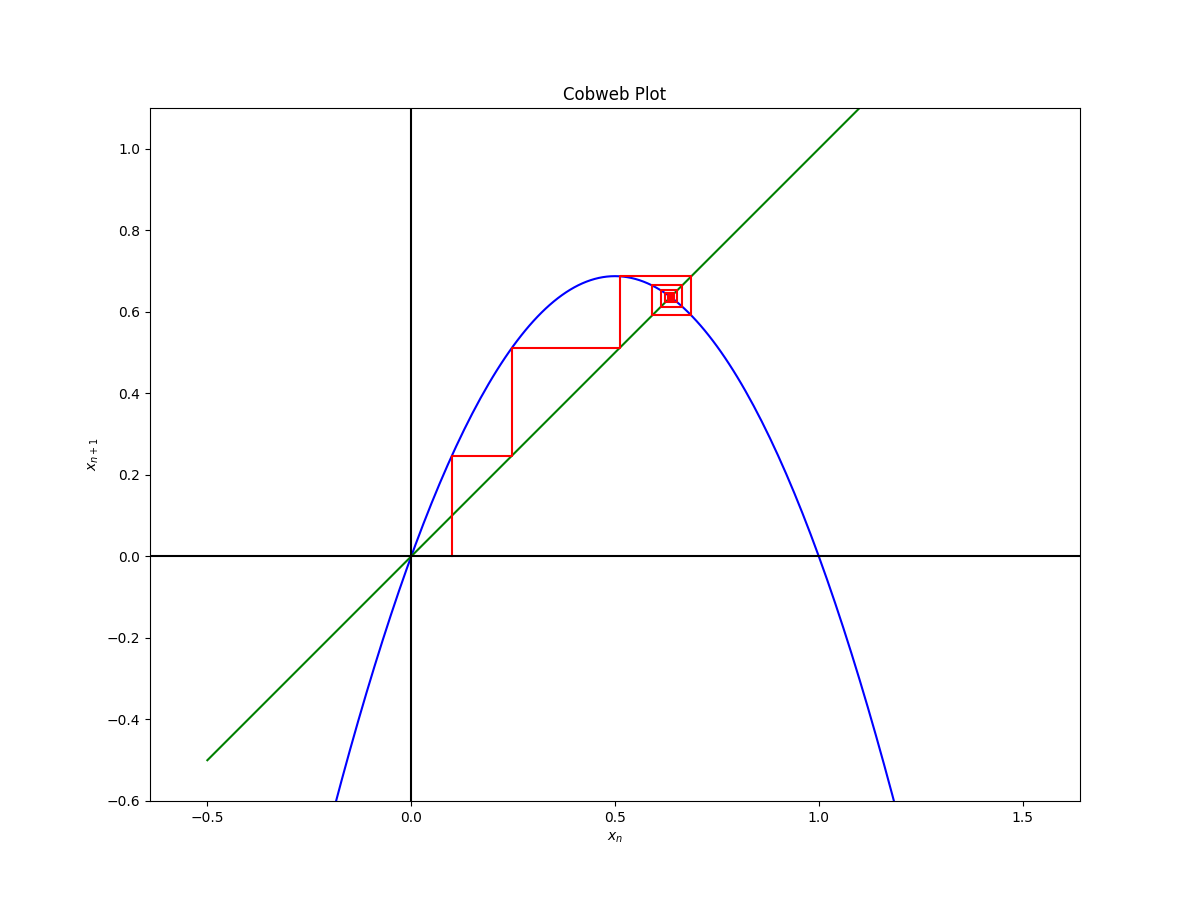
\includegraphics[scale = 0.4]{cobweb_01}
	\caption{Cobweb plot of $x_{t + 1} = x_t r (1 - x_t)$}
	\label{fig:cobweb_01}
\end{figure}\medskip

One technique for helping us to understand non-linear discrete models is
\emph{cobwebbing}, which is a graphical method for finding equilibrium points. The
technique is as follows: \bigskip

\begin{itemize}
	\item construct a set of axes with $x_t$ along the horizontal and $x_{t + 1}$ along the vertical
	\item draw the curve of the function $x_{t + 1} = f(x_t)$
	\item draw the line $x_{t + 1} = x_t$
	\item draw a line vertically up from $(x_0, 0)$ on the horizontal till it meets the curve of the function
	\item this point is $(x_0, x_1)$
	\item draw a line horizontally from $(x_0, x_1)$ till it meets the line $x_{t + 1} = x_t$
	\item call this point $(x_1, x_1)$
	\item with this point we repeat the above process until we either converge to an equilibrium point or diverge
\end{itemize}\medskip

Equilibrium points are located where the curve and the line intersect - usually denoted $x^*$. \bigskip









\chapter{Discrete Logistic Growth}




\section{Basics}

Consider the Logistic growth model: \bigskip

\[
	\frac{dN}{dt} = r N \Bigg( 1 - \frac{N}{K} \Bigg)
\]\medskip

where $r$ is the growth rate, and $K$ is the carrying capacity. We can turn this into a
discrete model as follows: \bigskip

\begin{eqnarray*}
    N_{t + 1} - N_t & = & r N_t \Bigg( 1 - \frac{N_t}{K} \Bigg) \\
          N_{t + 1} & = & N_t + r N_t \Bigg( 1 - \frac{N_t}{K} \Bigg) \\
                    & = & N_t \Bigg( 1 + r - \frac{r N_t}{K} \Bigg) \\
                    & = & N_t (1 + r) \Bigg( 1 - \frac{r N_t}{(1 + r) K} \Bigg)
\end{eqnarray*}\medskip

by making a transformation we have: \bigskip

\[
    x_{t + 1} = f(x_t) = x_t r' (1 - x_t) \quad \text{ where } \quad r' = 1 + r  \quad \text{ and }  \quad x_t = \frac{r N_t}{(1 + r) K}
\]\medskip




\section{Equilibrium}

we now investigate the equilibrium states of this model, with $0 \le r \le 4$ for
simplicity: \bigskip

\begin{eqnarray*}
         x^* & = & x^* r (1 - x^*) \\
 r (1 - x^*) & = & 1 \\
     1 - x^* & = & \frac{1}{r} \\
         x^* & = & \frac{r - 1}{r}
\end{eqnarray*}\medskip

so we have two equilibrium points - $x^* = 0$ and $x^* = (r - 1)/r$ with $r > 1$ (as we
are not interested in negative populations). In order to understand the behaviour of the
equilibrium points we need to look at the first derivative of $f(x)$: \bigskip

\begin{eqnarray*}
   f(x) & = & x r (1 - x) \\
  f'(x) & = & r (1 - 2x)
\end{eqnarray*}\medskip




\section{Stability}

Examining both these equilibrium points with $\left| f'(x) \right| < 1$ denoting stability,
and $\left| f'(x) \right| > 1$ denoting instability: \bigskip

\begin{eqnarray*}
                            f'(0) & = & r \\
    f'\bigg(\frac{r - 1}{r}\bigg) & = & 2 - r
\end{eqnarray*}\medskip

so $x^* = 0$ is stable for $r < 1$, and unstable for $r > 1$, and $x^* = (r - 1) / r$ is stable for $1 < r < 3$,
and does not exist for $0 < r < 1$: \bigskip

\begin{table}[h!]
	\centering
	\bgroup
	\setlength{\tabcolsep}{20pt}
	\def\arraystretch{2}
	\begin{tabular}{ c | c | c }
		                        & $0 < r < 1$    & $1 < r < 3$ \\
		\hline
		$x^* = 0$               & stable         & unstable \\
		\hline
		$x^* = \frac{r - 1}{r}$ & does not exist & stable
	\end{tabular}
    \egroup
	\caption{Stability of discrete logistic growth model}
	\label{table:logit}
\end{table}\medskip




\section{Chaos}

$r = 1$ and $r = 3$ are known as \emph{bifurcation points} and represent parameter values where
our model's behaviour changes. In order to understand the model's behaviour for $r > 3$ first we
observe the following: \bigskip

\begin{eqnarray*}
    x_{t + 1} & = & f(x_t) \\
              & = & f(f(x_{t - 1})) = f^2(x_{t - 1}) \\
              & = & f^2(f(x_{t - 2})) = f^3(x_{t - 2}) \\
              & \mathrel{\makebox[\widthof{=}]{\vdots}} \\
              & = & f^{t + 1}(x_0)
\end{eqnarray*}\medskip

and in particular, looking at the second order difference equation: \bigskip

\begin{eqnarray*}
    x_{t + 2} & = & f^2(x_t) \\
              & = & f(f(x_t)) \\
              & = & f(x_t) r (1 - f(x_t)) \\
              & = & x_t r^2 (1 - x_t) (1 - x_t r (1 - x_t))
\end{eqnarray*}\medskip

setting $x_{t + 2} = x_t = x^*$ we find: \bigskip

\begin{eqnarray*}
     x^* & = & x^* r^2 (1 - x^*) (1 - x^* r (1 - x^*)) \\
       1 & = & r^2 (1 - x^*) (1 - x^* r (1 - x^*)) \\
       1 & = & r^2 (1 - x^* r + (x^*)^2 r - x^* + (x^*)^2 r - (x^*)^3 r) \\
       1 & = & r^2 - x^* r^3 + (x^*)^2 r^3 - x^* r^2 + (x^*)^2 r^3 - (x^*)^3 r^3 \\
       0 & = & 1 - r^2 + x^* r^3 - (x^*)^2 r^3 + x^* r^2 - (x^*)^2 r^3 + (x^*)^3 r^3
\end{eqnarray*}\medskip

after some manipulation this reduces to: \bigskip

\[
    (r x^* - (r + 1))(r^2 (x^*)^2 - r (r + 1) x^* + (r + 1)) = 0
\]\medskip

\begin{figure}[t]
	\centering
	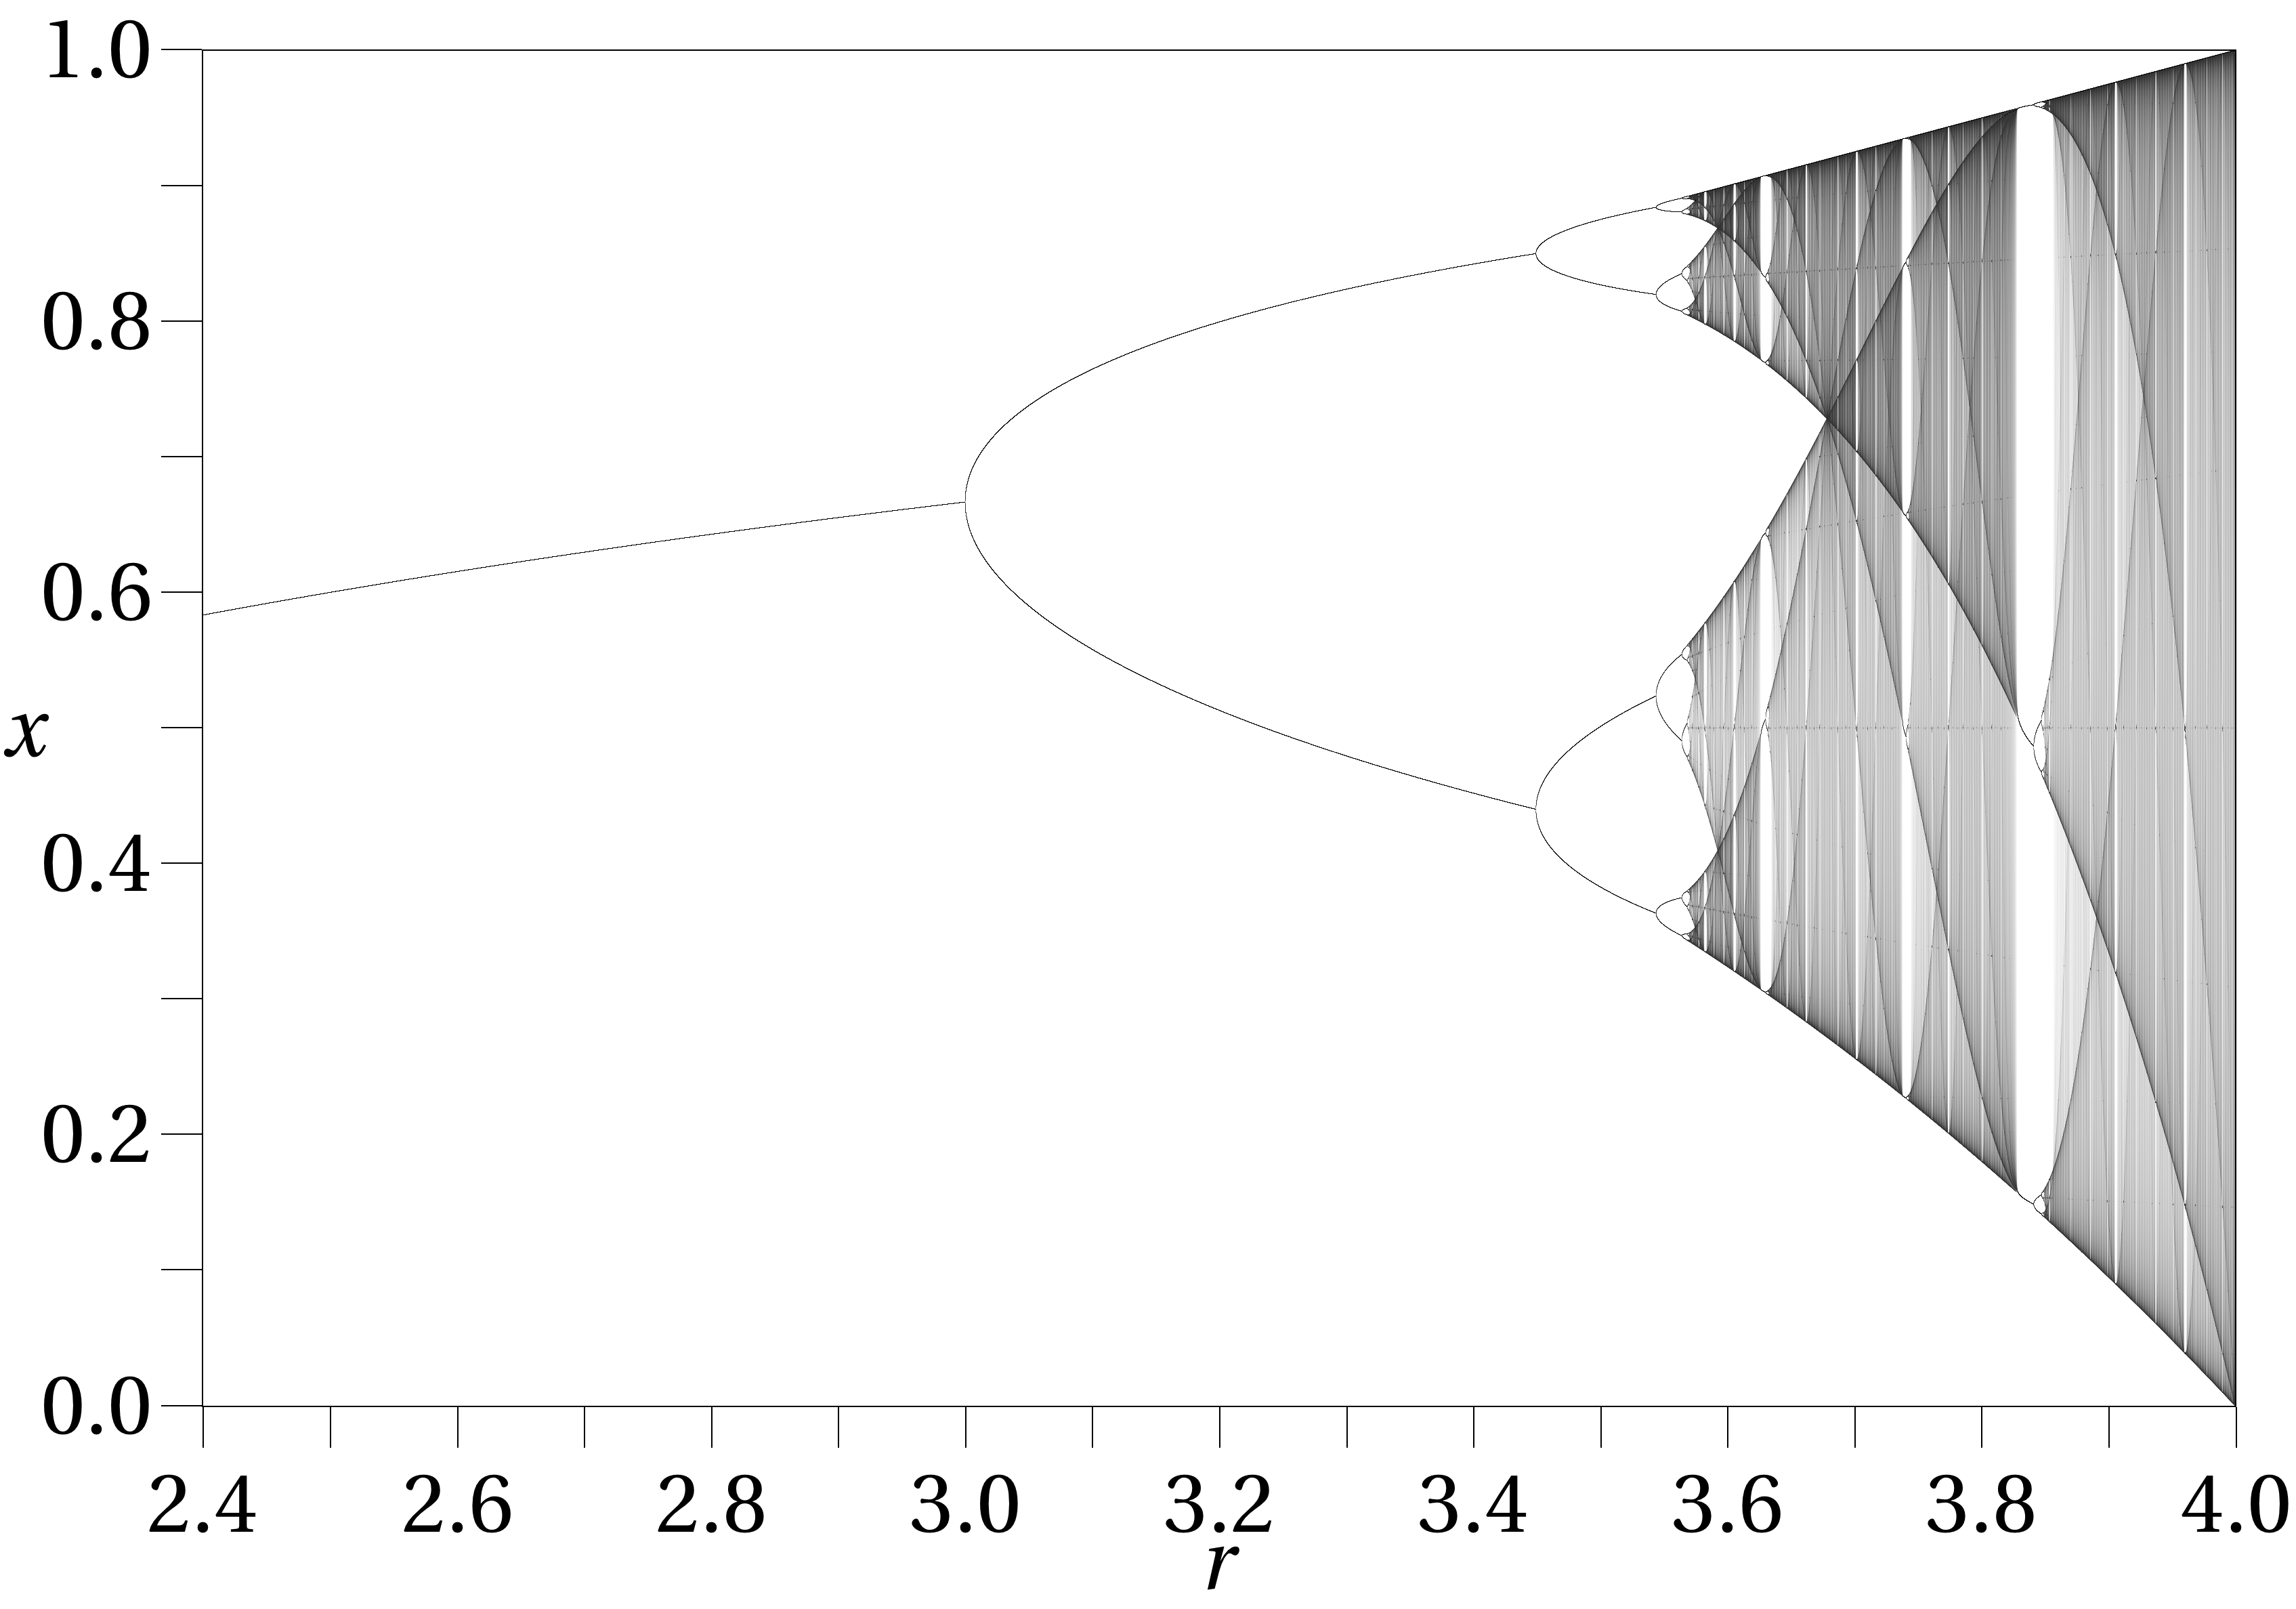
\includegraphics[scale = 0.10]{logistic_bifurcation}
	\caption{Bifurcations}
	\label{fig:bifurcations}
\end{figure}\medskip

here $r x^* - (r + 1) = 0$ gives us one of our original equilibrium points, so instead we
look at: \bigskip

\[
    r^2 (x^*)^2 - r (r + 1) x^* + (r + 1) = 0
\]\medskip

this quadratic will give us two real roots if the discriminant is positive: \bigskip

\begin{eqnarray*}
     r^2 (r + 1)^2 - 4 r^2 (r + 1) & > & 0 \\
           r^2 + 2 r + 1 - 4 r - 4 & > & 0 \\
                     r^2 - 2 r - 3 & > & 0 \\
                   (r + 1) (r - 3) & > & 0
\end{eqnarray*}\medskip

as we have restricted ourselves to $r > 0$, we have $r > 3$, and our solutions are: \bigskip

\[
	x^* = \frac{(r + 1) \pm \sqrt{(r + 1) (r - 3)}}{2 r}
\]\medskip

so the next solution is said to have period $2$ as there are two possible values. This process
continues for increasing $r$. So $p$-periodic solutions become $2p$-periodic solutions, and so
on. \bigskip

If an odd periodic solution ($p \ge 3$) exists for some value of $r$, say $r_c$, then there
is said to be \emph{aperiodic} or \emph{chaotic} solutions for $r > r_c$. Chaotic solutions are
solutions that oscillate in random, or unpredictable, ways.\bigskip




\section{Analysis}

We now investigate the stability of our Logistic growth model analytically through
linearisation about an equilibrium point: \bigskip

\[
    x_t = x^* + u_t, \qquad \left|u_t\right| \ll 1
\]\medskip

substituting this into our function we get: \bigskip

\[
    x^* + u_{t + 1} = f(x^* + u_t)
\]\medskip

Taylor expanding around the equilibrium point we get: \bigskip

\[
    x^* + u_{t + 1} = f(x^*) +  u_t f'(x^*) + \mathcal{O}(u_t^2), \qquad \left|u_t\right| \ll 1
\]\medskip

as $x^*$ is an equilibrium point, $f(x^*) = x^*$, and discarding higher powers of $u_t$,
we get: \bigskip

\begin{eqnarray*}
    u_{t + 1} & = & u_t f'(x^*) \\
              & = & \lambda u_t \\
              & = & \lambda^{t + 1} u_0
\end{eqnarray*}\medskip

where $\lambda = f'(x^*)$. From this we can draw conclusions about the stability of the
equilibrium point. It is clear that: \bigskip

\begin{eqnarray*}
    \left| \lambda \right| < 1 & \implies & \lim_{t \to \infty} u_t = 0 \\
    \left| \lambda \right| > 1 & \implies & \lim_{t \to \infty} u_t = \pm \infty
\end{eqnarray*}\medskip

and hence: \bigskip

\begin{eqnarray*}
	\left| f'(x^*) \right| < 1 & \implies & x^* \quad \text{ is stable } \\
	\left| f'(x^*) \right| > 1 & \implies & x^* \quad \text{ is unstable }
\end{eqnarray*}\medskip









\chapter{Discrete Models with Delay}




\section{Introduction}

So far we have assumed that all members of the population at time $t$ contribute to the
population at time $t + 1$, but this is not always the case. For example, depending upon
the interval of time, some members of a population may not have yet reached sexual
maturity, and hence cannot contribute to the population. As a consequence it makes sense
in some cases to introduce a delay term to the model. \bigskip

\[
    x_{t + 1} = f(x_t, x_{t - \tau})
\]\medskip




\section{Analysis}

We switch now to a different model - Ricker's model: \bigskip

\[
    x_{t + 1} = x_t \exp(r (1 - x_t))
\]\medskip

with $r > 0$ - which has equilibrium points $x^* = 0$ and $x^* = 1$. We make a slight
change to this model by introducing a delay term: \bigskip

\[
    x_{t + 1} = x_t \exp(r (1 - x_{t - 1}))
\]\medskip

again, with $r > 0$. Now we linearise around $x^* = 1$:\bigskip

\[
    x_t = 1 + u_t, \qquad \left|u_t\right| \ll 1
\]\medskip

substituting into our equation above we get: \bigskip

\begin{eqnarray*}
    1 + u_{t + 1} & = & (1 + u_t) \exp(r (1 - (1 + u_{t - 1}))) \\
                  & = & (1 + u_t) \exp(-r u_{t - 1}) \\
                  & \approx & (1 + u_t) (1 - r u_{t - 1}) \\
                  & = & 1 - r u_{t - 1} + u_t - r u_t u_{t - 1} \\
        u_{t + 1} & = & u_t - r u_{t - 1}
\end{eqnarray*}\medskip

the above using the fact that $\exp(x) \approx 1 + x$ for small $x$. \bigskip




\section{Solutions}

We have reduced our model to a second order difference equation: \bigskip

\[
    u_{t + 1} - u_t + r u_{t - 1} = 0
\]\medskip

with characteristic equation: \bigskip

\[
    z^2 - z + r = 0
\]\medskip

with solutions: \bigskip

\begin{eqnarray*}
    z_{1, 2} & = & \frac{1}{2} \Big[ 1 \pm \sqrt{1 - 4 r} \Big] \qquad 0 < r < \frac{1}{4} \\
    z_{1, 2} & = & \frac{1}{2} \Big[ 1 \pm i \sqrt{4 r - 1} \Big] \qquad \frac{1}{4} < r < 1
\end{eqnarray*}\medskip

for the case of $0 < r < \frac{1}{4}$ we have: \bigskip

\[
    u_t = C_1 z_1^t + C_2 z_2^t
\]\medskip

and because $0 < z_{1, 2} < 1$: \bigskip

\[
    \lim_{t \to \infty} u_t = 0
\]\medskip

and hence: \bigskip

\[
    \lim_{t \to \infty} x_t = 1
\]\medskip

therefore $x^* = 1$ is stable for $0 < r < \frac{1}{4}$. For the case of $\frac{1}{4} < r < 1$
we have: \bigskip

\begin{eqnarray*}
      \rho & = & \left| z_{1, 2} \right| = \sqrt{r} \\
    \theta & = & \tan^{-1}(\sqrt{4 r - 1}) \\
  z_{1, 2} & = & \rho e^{\pm i \theta}
\end{eqnarray*}\medskip

which leads to: \bigskip

\begin{eqnarray*}
    u_t & = & C z^t + \overline{C} \overline{z}^t \\
        & = & \left| A \right| e^{i \gamma} (\rho e^{i \theta})^t + \left| A \right| e^{-i \gamma} (\rho e^{- i \theta})^t \\\\
        & = & 2 \left| A \right| \rho^t \Bigg(\frac{e^{i (\theta t + \gamma)} + e^{- i (\theta t + \gamma)}}{2}\Bigg) \\\\
        & = & 2 \left| A \right| \rho^t \cos(\theta t + \gamma)
\end{eqnarray*}\medskip

which is stable as $r < 1$. If we take $r_c = 1$, then at $r_c$ we have: \bigskip

\begin{eqnarray*}
    \theta_c & = & \tan^{-1}(\sqrt{4 r_c - 1}) \\
             & = & \tan^{-1}(\sqrt{3}) \\
             & = & \frac{\pi}{3}
\end{eqnarray*}\medskip

from which we get: \bigskip

\[
    u_t = 2 \left| A \right| \cos(\frac{\pi}{3} t + \gamma)
\]\medskip

and hence: \bigskip

\begin{eqnarray*}
    \frac{\pi}{3} t_p & = & 2 \pi \\
                  t_p & = & 6
\end{eqnarray*}\medskip

and for $r > r_c$ we have $\rho > 1$ which gives us: \bigskip

\[
    \lim_{t \to \infty} u_t = \pm \infty
\]\medskip

and hence: \bigskip

\[
    \lim_{t \to \infty} x_t = \pm \infty
\]\medskip









\chapter{Solutions to problems}



\section{$x_{n + 1} = \beta x_n + \alpha x_{n - 1}$}

This is a linear system. The solution is as follows: \bigskip

\begin{eqnarray*}
                                   x_{n + 1} & = & \beta x_n + \alpha x_{n - 1} \\
    x_{n + 1} - \beta x_n - \alpha x_{n - 1} & = & 0
\end{eqnarray*}\medskip

with characteristic equation: \bigskip

\[
    \lambda^2 - \beta \lambda - \alpha = 0
\]\medskip

and solutions: \bigskip

\[
    \lambda_{1, 2} = \frac{\beta \pm \sqrt{\beta^2 + 4 \alpha}}{2}
\]\medskip

our general solution is of the form: \bigskip

\[
    x_n = C_1 \lambda_1^n + C_2 \lambda_2^n
\]\medskip

which gives us for $n = 0$ and $n = 1$: \bigskip

\begin{eqnarray*}
    x_0 & = & C_1 + C_2 \\
    x_1 & = & C_1 \lambda_1 + C_2 \lambda_2
\end{eqnarray*}\medskip

taking $x_1$ we get: \bigskip

\begin{eqnarray*}
        x_1 & = & C_1 \frac{\beta + \sqrt{\beta^2 + 4 \alpha}}{2} + C_2 \frac{\beta - \sqrt{\beta^2 + 4 \alpha}}{2} \\
            & = & \frac{\beta}{2} (C_1 + C_2) + \frac{\sqrt{\beta^2 + 4 \alpha}}{2} (C_1 - C_2) \\
            & = & \frac{\beta}{2} x_0 + \frac{\sqrt{\beta^2 + 4 \alpha}}{2} (C_1 - C_2) \\\\
  C_1 - C_2 & = & \frac{2 x_1 - \beta x_0}{\sqrt{\beta^2 + 4 \alpha}} \\
  C_1 + C_2 & = & x_0
\end{eqnarray*}\medskip

solving for $C_1$ and $C_2$ we get: \bigskip

\begin{eqnarray*}
	C_1 & = & \frac{ x_0 (\sqrt{\beta^2 + 4 \alpha} - \beta) + 2 x_1  }{ 2 \sqrt{\beta^2 + 4 \alpha}  } \\\\
	C_2 & = & \frac{ x_0 (\sqrt{\beta^2 + 4 \alpha} + \beta) - 2 x_1  }{ 2 \sqrt{\beta^2 + 4 \alpha}  }
\end{eqnarray*}\medskip

so our general solution is: \bigskip

\begin{eqnarray*}
    x_n = \Bigg(\frac{x_0 (\sqrt{\beta^2 + 4 \alpha} - \beta) + 2 x_1}{2 \sqrt{\beta^2 + 4 \alpha}}\Bigg)
          \Bigg(\frac{\beta + \sqrt{\beta^2 + 4 \alpha}}{2}\Bigg)^n \\\\
          + \Bigg(\frac{x_0 (\sqrt{\beta^2 + 4 \alpha} + \beta) - 2 x_1}{2 \sqrt{\beta^2 + 4 \alpha}}\Bigg)
            \Bigg(\frac{\beta - \sqrt{\beta^2 + 4 \alpha}}{2}\Bigg)^n
\end{eqnarray*}\medskip







%\section{$x_{n + 1} = \frac{x_n}{1 + x_n}$}
\section{$x_{n + 1} = \sfrac{x_n}{1 + x_n}$}

This is a non-linear system. \bigskip

\[
    x_{n + 1} = \frac{x_n}{1 + x_n}
\]\medskip

finding the equilibrium points: \bigskip

\begin{eqnarray*}
                      x^* & = & \frac{x^*}{1 + x^*} \\\\
    \therefore \qquad x^* & = & 0
\end{eqnarray*}\medskip

now we look at the stability: \bigskip

\begin{eqnarray*}
    f(x) & = & \frac{x}{1 + x} \\
   f'(x) & = & \frac{1}{(1 + x)^2} \\\\
   f'(0) & = & 1
\end{eqnarray*}\medskip

therefore, strictly speaking, we cannot say that $x^* = 0$ is either stable or unstable.
Looking at the system graphically (Figure \ref{fig:cobweb_02}) starting in the
neighbourhood of $1$ and cobwebbing,  we see that the system tends towards $0$ which
would imply $x^* = 0$ is stable. \bigskip

\begin{figure}[h]
	\centering
	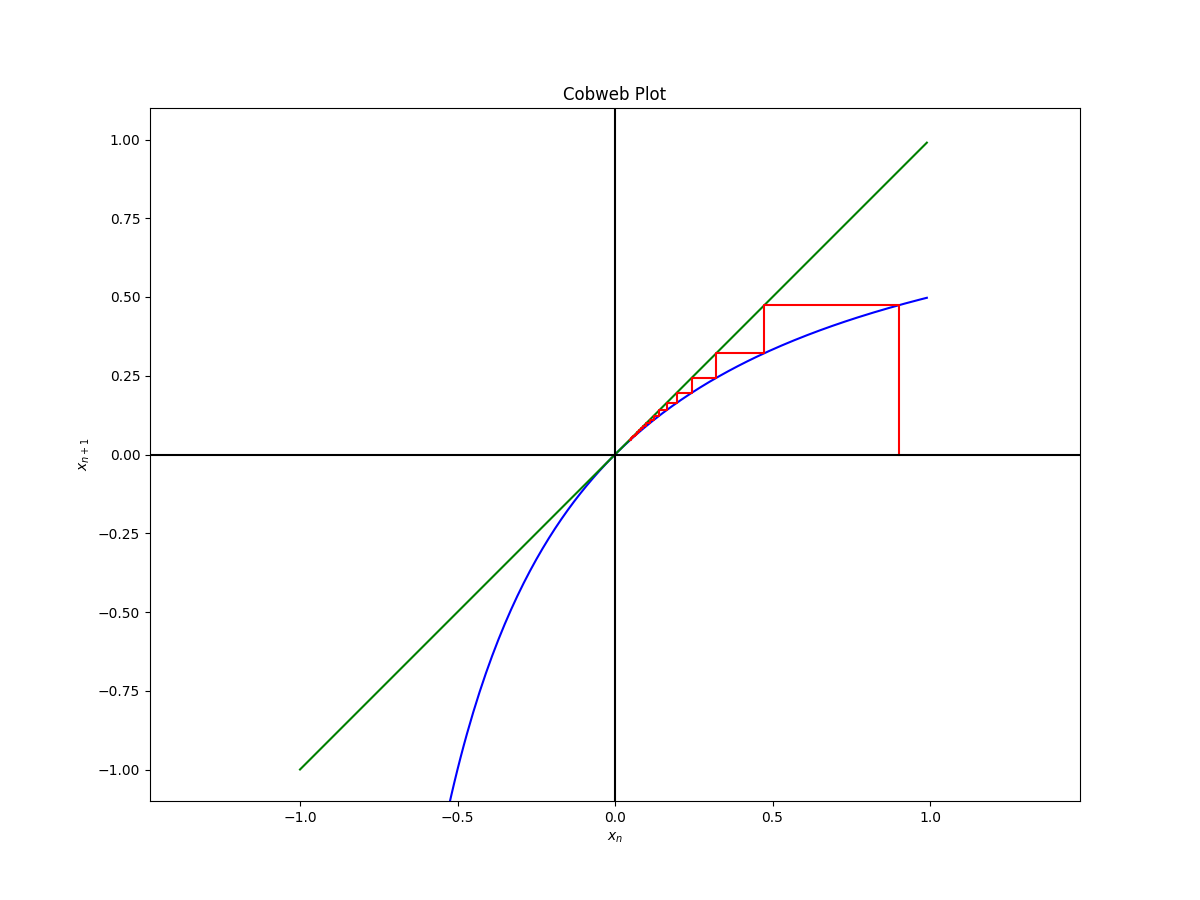
\includegraphics[scale = 0.4]{cobweb_02}
	\caption{Cobweb plot of $x_{n + 1} = \sfrac{x_n}{1 + x_n}$}
	\label{fig:cobweb_02}
\end{figure}\medskip



%But what may be of interest is looking at the limit of the sequence: \bigskip
%
%\[
%    \lim_{n \to \infty} x_n = 1
%\]\medskip
%
%we see that: \bigskip
%
%\[
%    f'(1) = \frac{1}{4}
%\]\medskip
%
%which is stable. \bigskip







%\section{$x_{n + 1} = \frac{1}{2 + x_n}$}
\section{$x_{n + 1} = \sfrac{1}{2 + x_n}$}

This is a non-linear system. \bigskip

\[
    x_{n + 1} = \frac{1}{2 + x_n}
\]\medskip

finding the equilibrium points: \bigskip

\begin{eqnarray*}
                             x^* & = & \frac{1}{2 + x^*} \\
                 2 x^* + (x^*)^2 & = & 1 \\
             (x^*)^2 + 2 x^* - 1 & = & 0 \\\\
                      \qquad x^* & = & -1 \pm \sqrt{2}
\end{eqnarray*}\medskip

now we look at the stability: \bigskip

\begin{eqnarray*}
                            f(x) & = & \frac{1}{2 + x} \\
                           f'(x) & = & \frac{-1}{(2 + x)^2} \\\\
\left| f'(-1 + \sqrt{2}) \right| & < & 1 \\
\left| f'(-1 - \sqrt{2}) \right| & > & 1
\end{eqnarray*}\medskip

therefore $x^* = -1 + \sqrt{2}$ is stable, and $x^* = -1 - \sqrt{2}$ is unstable. \bigskip
% therefore the equilibrium point $x^* = -1 + \sqrt{2}$ is stable. \bigskip







\section{$x_{n + 1} = x_n e^{\alpha x_n}$}

This is a non-linear system. \bigskip

\[
    x_{n + 1} = x_n e^{\alpha x_n}
\]\medskip

finding the equilibrium points: \bigskip

\begin{eqnarray*}
                       x^* & = & x^* e^{\alpha x^*} \\
     \therefore \qquad x^* & = & 0
\end{eqnarray*}\medskip

now we look at the stability: \bigskip

\begin{figure}[h]
	\centering
	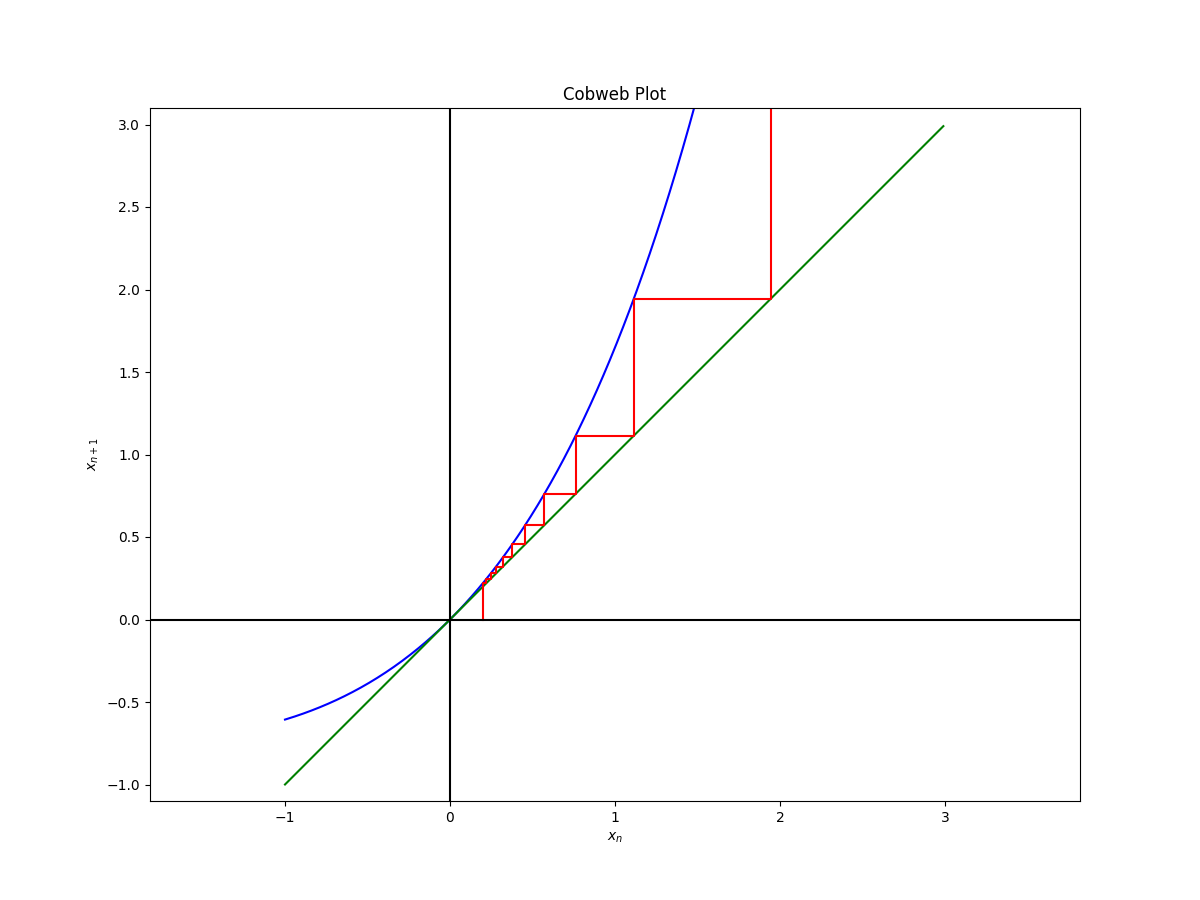
\includegraphics[scale = 0.4]{cobweb_03}
	\caption{Cobweb plot of $x_{n + 1} = x_n e^{\alpha x_n}$}
	\label{fig:cobweb_03}
\end{figure}\medskip

\begin{eqnarray*}
     f(x) & = & x e^{\alpha x} \\
    f'(x) & = & (1 + \alpha x) e^{\alpha x} \\
	f'(0) & = & 1
\end{eqnarray*}\medskip

therefore, strictly speaking, we cannot say that $x^* = 0$ is either stable or unstable.
Looking at the system graphically (Figure \ref{fig:cobweb_03}) starting in the
neighbourhood of $0$ and cobwebbing, we see that the system tends towards $\infty$, i.e.
is unbounded, which would imply $x^* = 0$ is unstable. \bigskip











\section{$x_{n + 1} = x_n \ln(x_n^2)$}

This is a non-linear system. \bigskip

\[
    x_{n + 1} = x_n \ln(x_n^2)
\]\medskip

finding the equilibrium points: \bigskip



\begin{eqnarray*}
                      x^* & = & x^* \ln((x^*)^2) \\
                          & = & 2 x^* \ln(x^*) \\\\
               2 \ln(x^*) & = & 1 \\
                 \ln(x^*) & = & \frac{1}{2} \\
                      x^* & = & \sqrt{e} \\
    \therefore \qquad x^* & = & 0 \quad \text{or} \quad \sqrt{e}
\end{eqnarray*}\medskip

now we look at the stability: \bigskip

\begin{figure}[h]
	\centering
	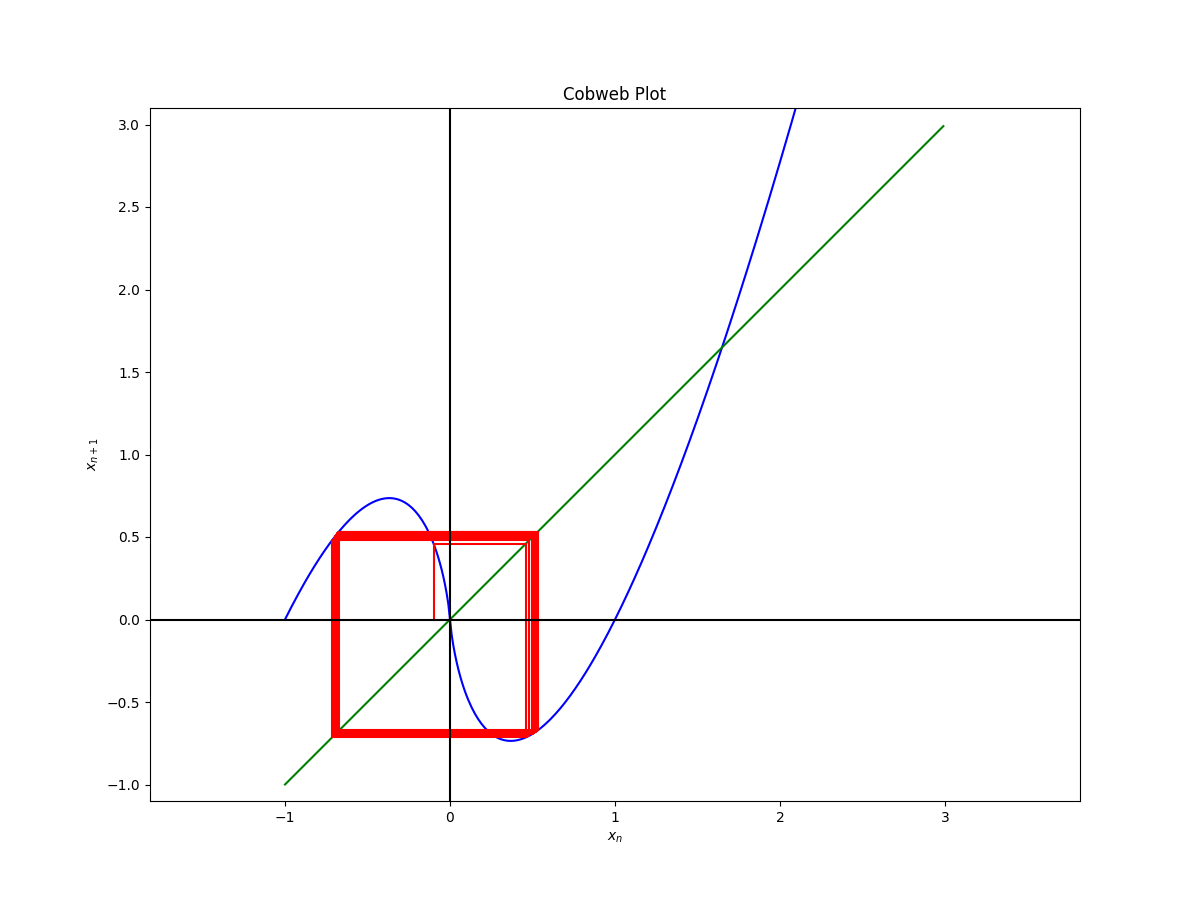
\includegraphics[scale = 0.4]{cobweb_04}
	\caption{Cobweb plot of $x_{n + 1} = x_n \ln(x_n^2)$ starting from $-0.1$}
	\label{fig:cobweb_04}
\end{figure}\medskip

\begin{figure}[h]
	\centering
	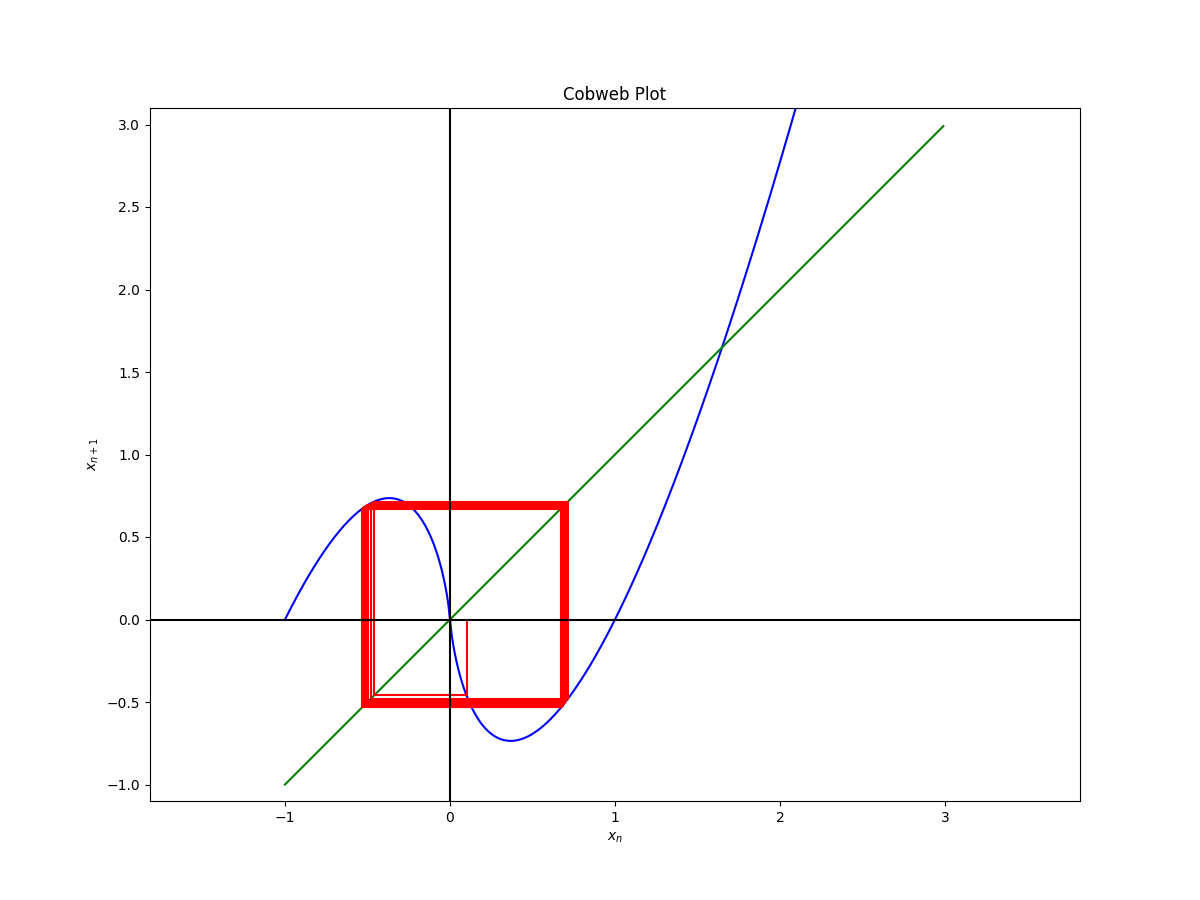
\includegraphics[scale = 0.4]{cobweb_05}
	\caption{Cobweb plot of $x_{n + 1} = x_n \ln(x_n^2)$ starting from $0.1$}
	\label{fig:cobweb_05}
\end{figure}\medskip

\begin{eqnarray*}
           f(x) & = & 2 x \ln(x) \\
          f'(x) & = & 2 (\ln(x) + 1) \\\\
          f'(0) & = & -\infty \\
   f'(\sqrt{e}) & = & 3
\end{eqnarray*}\medskip



therefore both $x^* = 0$ and $x^* = \sqrt{e}$ are unstable. But looking at the system
graphically and cobwebbing starting at $-0.1$ (Figure \ref{fig:cobweb_04}) and then
starting at $0.1$ (Figure \ref{fig:cobweb_05}) - i.e. in the neighbourhood of $0$ - we
see periodic oscillations that would suggest a periodic solutions to the system. \bigskip









\section{$(x_{n + 1} - \alpha)^2 = \alpha^2 (x_n^2 -2 x_n + 1)$}

This is a combination of linear systems. \bigskip

\begin{eqnarray*}
    (x_{n + 1} - \alpha)^2 & = & \alpha^2 (x_n^2 -2 x_n + 1) \\
                           & = & \alpha^2 (x_n - 1)^2 \\
        x_{n + 1} - \alpha & = & \pm \alpha (x_n - 1) \\
                 x_{n + 1} & = & \alpha \pm \alpha (x_n - 1) \\
                           & = & \alpha \pm (\alpha x_n - \alpha)
\end{eqnarray*}\medskip

this results in two linear systems, the first: \bigskip

\begin{eqnarray*}
    x_{n + 1} & = & \alpha x_n \\
              & = & \alpha^{n + 1} x_0
\end{eqnarray*}\medskip

and the second: \bigskip

\begin{eqnarray*}
    x_{n + 1} & = & 2 \alpha - \alpha x_n \\
              & = & 2 \alpha - \alpha (2 \alpha - \alpha x_{n - 1}) \\
              & = & 2 \alpha - 2 \alpha^2 + \alpha^2 x_{n - 1} \\
              & = & 2 \alpha - 2 \alpha^2 + \alpha^2 (2 \alpha - \alpha x_{n - 2}) \\
              & = & 2 \alpha - 2 \alpha^2 + 2 \alpha^3 - \alpha^3 x_{n - 2} \\
              & \mathrel{\makebox[\widthof{=}]{\vdots}} \\
\end{eqnarray*}

\begin{eqnarray*}
              & = & 2 \alpha \Big( \sum_{i = 0}^{n} (- \alpha)^i \Big) + (- \alpha)^{n + 1} x_0 \\\\
              & = & 2 \alpha \Big( \frac{1 - (- \alpha)^{n + 1}}{1 + \alpha} \Big) + (- \alpha)^{n + 1} x_0 \\\\
              & = & \Big( x_0 - \frac{2 \alpha}{1 + \alpha} \Big) (- \alpha)^{n + 1} + \frac{2 \alpha}{1 + \alpha} \\\\
              & = & (-1)^{n + 1} \Big( x_0 - \frac{2 \alpha}{1 + \alpha} \Big) \alpha^{n + 1} + \frac{2 \alpha}{1 + \alpha}
\end{eqnarray*}\medskip

both systems converge for $\left| \alpha \right| < 1$, the first system converges to
$0$, the second to $2 \alpha / 1 + \alpha$. \bigskip

%finding the equilibrium points: \bigskip
%
%\begin{eqnarray*}
%         (x^* - \alpha)^2 & = & \alpha^2 ((x^*)^2 - 2 x^* + 1) \\
%                          & = & \alpha^2 (x^* - 1)^2 \\
%             x^* - \alpha & = & \pm \alpha (x^* - 1) \\
%                      x^* & = & \alpha \pm \alpha (x^* - 1) \\\\
%                      x^* & = & \alpha x^* \\
%                      x^* & = & 2 \alpha - \alpha x^* \\\\
%    \therefore \qquad x^* & = & 0 \qquad \text{or} \qquad \frac{2 \alpha}{1 + \alpha}
%\end{eqnarray*}\medskip
%
%as an aside, taking a longer approach: \bigskip
%
%\begin{eqnarray*}
%                                              (x^* - \alpha)^2 & = & \alpha^2 ((x^*)^2 - 2 x^* + 1) \\
%                             (x^*)^2 - 2 \alpha x^* + \alpha^2 & = & \alpha^2 (x^*)^2 - 2 \alpha^2 x^* + \alpha^2 \\
%    (x^*)^2 - 2 \alpha x^* - \alpha^2 (x^*)^2 + 2 \alpha^2 x^* & = & 0 \\
%              x^* (x^* - \alpha^2 x^* - 2 \alpha + 2 \alpha^2) & = & 0 \\
%              x^* (x^* (1 - \alpha^2) - 2 \alpha (1 - \alpha)) & = & 0 \\\\
%                                         \therefore \qquad x^* & = & 0 \quad \text{or} \quad \frac{2 \alpha}{1 + \alpha}
%\end{eqnarray*}\medskip
%
% Now we look at the stability:
%now we look at the stability: \bigskip
%
%\begin{eqnarray*}
%     f(x) & = & \alpha \pm \alpha (x - 1) \\
%    f'(x) & = & \pm \alpha
%\end{eqnarray*}\medskip
%
%hence the stability is completely dependent upon the parameter $\alpha$. So for
%stability we must have: \bigskip
%
%\[
%    \left| \alpha \right| < 1
%\]\medskip







\section{$x_{n + 1} = \sqrt{x_n + 2}$}

This is a non-linear system. \bigskip

\[
    x_{n + 1} = \sqrt{x_n + 2}
\]\medskip

finding the equilibrium points: \bigskip

\begin{eqnarray*}
                      x^* & = & \sqrt{x^* + 2} \\
                  (x^*)^2 & = & x^* + 2 \\
        (x^*)^2 - x^* - 2 & = & 0 \\\\
    \therefore \qquad x^* & = & -1 \quad \text{or} \quad 2
\end{eqnarray*}\medskip

we discard $x^* = -1$ as it is not positive. Now we look at the
stability of $x^* = 2$: \bigskip

\begin{eqnarray*}
     f(x) & = & \sqrt{x + 2} \\
    f'(x) & = & \frac{1}{2 \sqrt{x + 2}} \\\\
   % f'(-1) & = & \frac{1}{2} \\\\
    f'(2) & = & \frac{1}{4} \\
\end{eqnarray*}\medskip

therefore the equilibrium point $x^* = 2$ is stable. \bigskip





%\cite{book1, book2}

\newpage








\bibliographystyle{plain}
\bibliography{bibtex/bibliography}

\end{document}
